\chapter{Performance}\label{chap:performance}

\section{Complexity}

Most of operations in \gravity are AES rounds, through AES-256-CTR, Haraka-256, or Haraka-512. 
AES-256-CTR does 14 AES rounds per 16-byte block generated.
Haraka-256 does 24 AES rounds per 32-byte value hashed, and Haraka-512 does 48 rounds per 64-byte value hashed.
% TODO: check these 24 and 48

Table~\ref{tab:complexity} gives the count of these operations for each \gravity instance, where
\begin{itemize}
    \item Key generation needs $100T- 48C$ AES rounds

    \item Signature needs $100T - 48C + 7K + 96$ AES rounds, where we count $8K$ bytes for subset generation, as in our reference code (thus $K/2$ AES calls, or $7K$ rounds)
    
    \item Verification needs $K(24 + 48(\log T - \log C) + 7K + 48$ AES rounds
\end{itemize}

We ignore the cost of hashing the message with \hashx, and we also ignore the potential speed-up of pipelined or parallel computation of AES rounds.

\begin{table}
\centering 
\begin{tabular}{cc|ccc|c}
\toprule
Operation & ID & AES-256 & Haraka-256 & Haraka-512 & AES rounds \\
\midrule
\multirow{3}{*}{Key generation}
& S & $\num{262144}$ & $\num{131072}$ & $\num{131008}$ & $\num{13104128}$ \\
& M & $\num{524288}$ & $\num{262144}$ & $\num{262016}$ & $\num{26208256}$ \\
& L & $\num{1048576}$ & $\num{524288}$ & $\num{524160}$ & $\num{52422656}$ \\
\midrule
\multirow{3}{*}{Signature}
& S & $\num{262171}$ & $\num{131072}$ & $\num{131010}$ & $\num{13104602}$ \\
&M & $\num{524319}$ & $\num{262144}$ & $\num{262018}$ & $\num{26208786}$ \\
&L & $\num{1048608}$ & $\num{524288}$ & $\num{524162}$ & $\num{52423200}$ \\
\midrule
\multirow{3}{*}{Verification} 
& S & 27 & 54 & $595$ & $\num{30234}$ \\
&M & 31 & 62 & $683$ & $\num{34706}$ \\
&L & 32 & 64 & $769$ & $\num{38896}$ \\
\bottomrule
\end{tabular}

\caption{Complexity of \gravity instances, counting the number of calls to each primitive. AES-256 does 14 rounds per block, Haraka-256 does 24 AES rounds, and Haraka-512 does 48. The count of AES-256 blocks for subset generation is an upper bound.}
\label{tab:complexity}
\end{table}

Verification is orders of magnitude faster than signature generation, which is ideal for the \gravity use cases: typically few signatures would be generated on powerful machines with no speed constraint, whereas verification may be performed multiple times on less powerful machines (for example, for firmware signatures or CA-issued certificates).

\section{Choosing a Number of Subtrees}\label{sec:tradeoff}

The number of substrees $C$ does not affect the security of the scheme, but allows to reduce the signature size by increasing the public key size: instead of including only the root of the tree (case $C=1$), the public key can include all the roots of subtrees at a lower level.

A larger $C$ also makes signature and verification slightly faster.

For the \gravity instances proposed, we choose the value of $C$ that minimizes the total length signature + public key. 
Other values of $C$ may be used to reduce the signature size or speed-up computations.

Figure~\ref{fig:subtrees} shows the different trade-offs for the proposed \gravity instances.

\begin{figure}
\centering
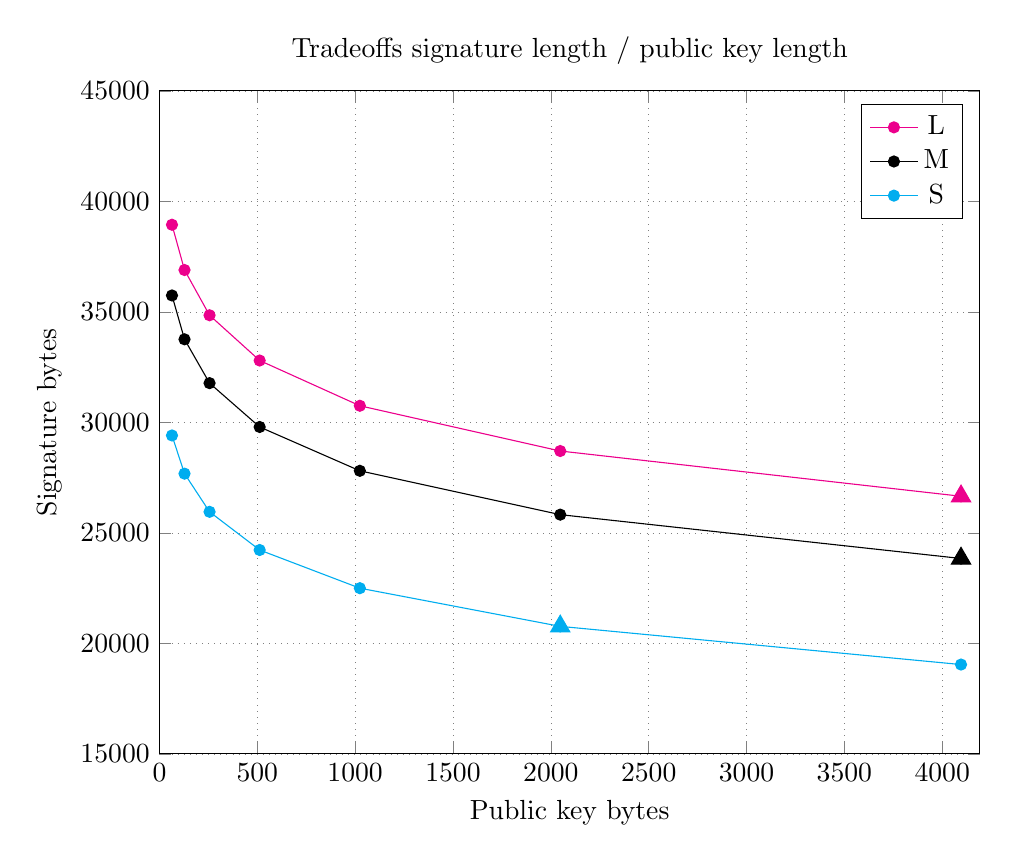
\begin{tikzpicture}
  \begin{axis}[title=Tradeoffs signature length / public key length,
    width=12cm,
    height=10cm,
    xlabel=Public key bytes,
    ylabel=Signature bytes,
    ytick distance=5000,
    xtick distance=500,
    xmin=0,
    xmax=4192,
    ymin=15000,
    ymax=45000,
    x tick label style={
      /pgf/number format/.cd,
      set thousands separator={}
    },
    scaled y ticks=false,
    y tick label style={
      /pgf/number format/.cd,
      set thousands separator={}
    },
    grid style={help lines,dotted},
    grid=major
  ]

\addplot[magenta,mark=*] coordinates {
(64, 38944.000000)
(128, 36896.000000)
(256, 34848.000000)
(512, 32800.000000)
(1024, 30752.000000)
(2048, 28704.000000)
(4096, 26656.000000)
};
\addlegendentry{L};
\addplot[black,mark=*] coordinates {
(64, 35744.000000)
(128, 33760.000000)
(256, 31776.000000)
(512, 29792.000000)
(1024, 27808.000000)
(2048, 25824.000000)
(4096, 23840.000000)
};
\addlegendentry{M};
\addplot[cyan,mark=*] coordinates {
(64, 29408.000000)
(128, 27680.000000)
(256, 25952.000000)
(512, 24224.000000)
(1024, 22496.000000)
(2048, 20768.000000)
(4096, 19040.000000)
};
\addlegendentry{S};
\addplot[only marks,mark=triangle*,mark size=4pt,magenta] coordinates {
(4096, 26656.000000)
};
\addplot[only marks,mark=triangle*,mark size=4pt,black] coordinates {
(4096, 23840.000000)
};
\addplot[only marks,mark=triangle*,mark size=4pt,cyan] coordinates {
(2048, 20768.000000)
};

  \end{axis}
\end{tikzpicture}


%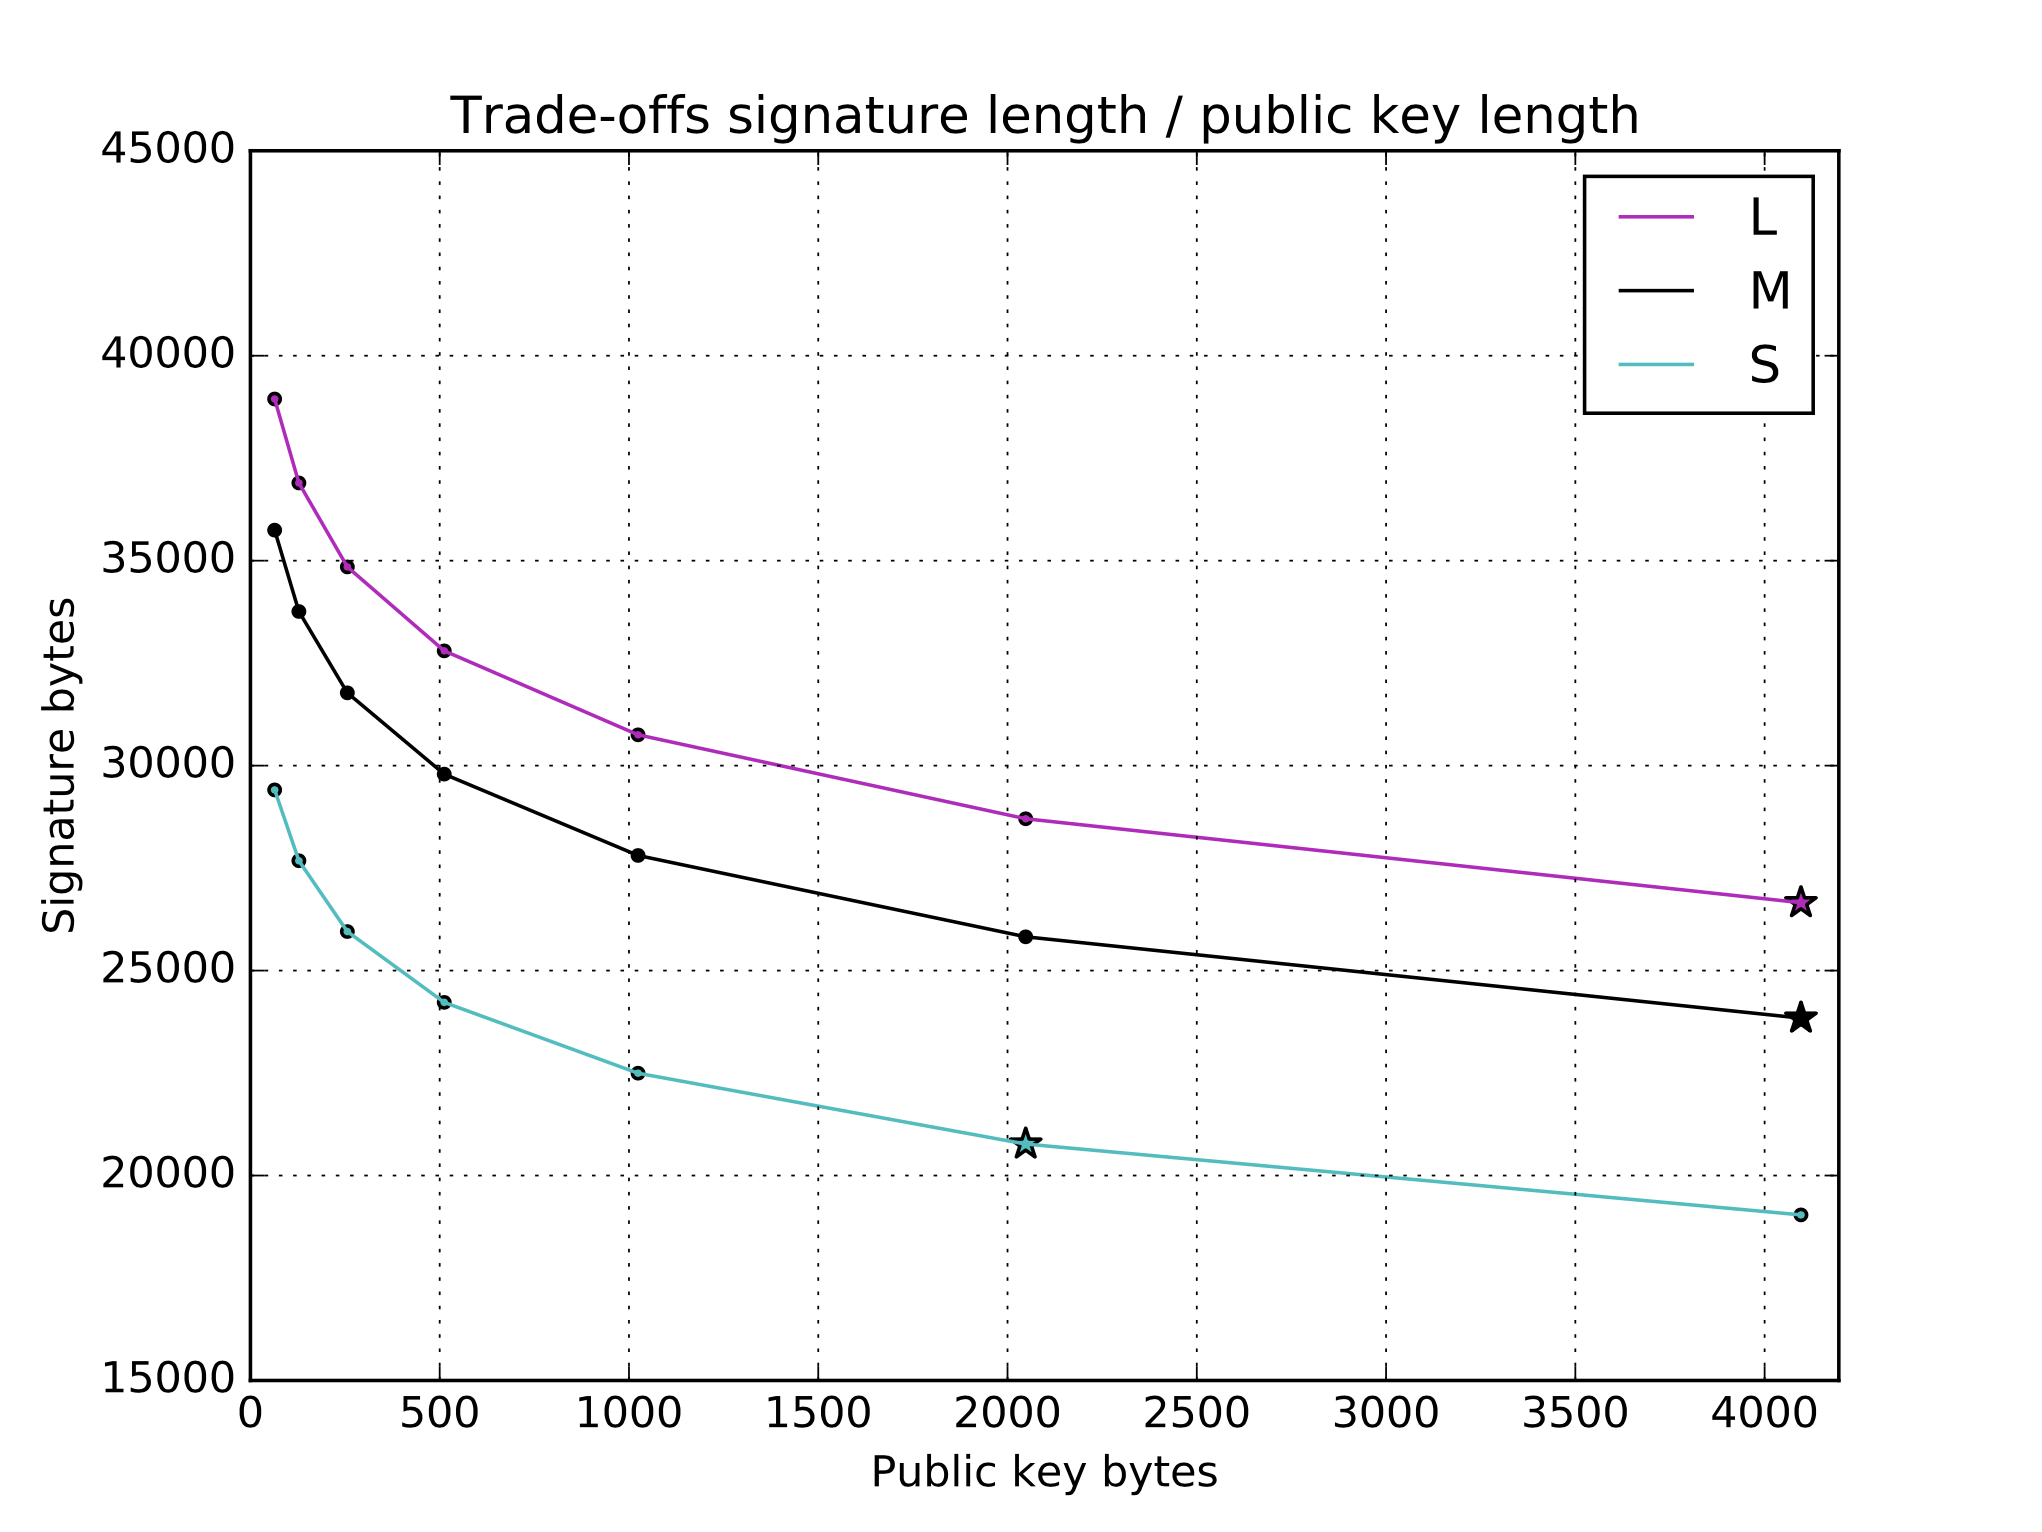
\includegraphics[width=14cm]{graph_subtrees}
\caption{Trade-offs between signature length and public-key length, for $C$ in $\{2^1, 2^2, \dots, 2^7\}$. The triangles indicate the optimal trade-offs, chosen for the instances proposed.}
\label{fig:subtrees}
\end{figure}


\section{Software Performance}

The AES rounds that constitute most of \gravity computations and the largest part of the execution time can be implemented with native AES instructions (AES-NI).

On Skylake CPUs, the AES round instruction AESENC has a latency of four cycles and a reciprocal throughput of one.
In \gravity, many AES rounds can be pipelined in order to maximize the effective throughput and return one AESENC result per cycle: Haraka-512 computes up to four independent AES rounds, and rounds within four AES-256-CTR instances can be interleaved.

These independent AES round instances can't really be parallelized on current microarchitectures that have a single AES unit. 
But AMD's new Ryzen CPUs have two AES units, and Intel is expect to follow in future microarchitectures versions and include two AES units as well.

Our optimized implementation thus includes 4-way and 8-way interleaved versions of Haraka for computing the trees and its leaves\footnote{Based on Haraka's authors code at \url{https://github.com/kste/haraka/}, with a few optimizations and bug fixes.}, as well as 4-way interleaved AES-256-CTR.

Signature verification requires only negligible memory: our implementation only allocates $140+K$ bytes on the stack, which is probably suboptimal. 

Our implementations of key generation and signing, however, allocate $32T$ heap bytes to store the subkeys and compute the tree.
This is respectively 4MiB, 8MiB, and 16MiB for instances S, M, and L.
But key generation and signing can be implemented to use much less memory, for example using techniques described in~\cite{armed}.

Below we report example results from running our benchmark program (\texttt{make bench}) on a Intel Core i7-6700 CPU @ 3.40GHz (Turbo Boost disabled), where the wall time is given in microseconds, and \texttt{crypto\_sign\_cached} implements the trick described in \S\S\ref{ssec:cache}:

Version S ($T=2^{17}, C=2^6, K=54$):
{\footnotesize
\begin{verbatim}
# crypto_sign_keypair
median cycles count:     14054574
average wall time:       4124.561 usec

# crypto_sign
median cycles count:     19551800
average wall time:       5747.488 usec

# crypto_sign_cached
median cycles count:     10418326
average wall time:       3063.229 usec

# crypto_sign_open
median cycles count:     72908
average wall time:       21.443 usec
\end{verbatim}
}

Version M ($T=2^{18}, C=2^7, K=62$):
{\footnotesize
\begin{verbatim}
# crypto_sign_keypair
median cycles count:     28193440
average wall time:       8276.869 usec

# crypto_sign
median cycles count:     40179136
average wall time:       11813.293 usec

# crypto_sign_cached
median cycles count:     20982546
average wall time:       6169.703 usec

# crypto_sign_open
median cycles count:     83650
average wall time:       24.598 usec
\end{verbatim}
}

Version L ($T=2^{19}, C=2^7, K=64$):
{\footnotesize
\begin{verbatim}

# crypto_sign_keypair
median cycles count:     58782818
average wall time:       17234.963 usec

# crypto_sign
median cycles count:     80689918
average wall time:       23750.260 usec

# crypto_sign_cached
median cycles count:     42442734
average wall time:       12473.613 usec

# crypto_sign_open
median cycles count:     93702
average wall time:       27.562 usec
\end{verbatim}
}
Note the low verification time for all instances (\texttt{crypto\_sign\_open}).


\section{Hardware Performance}

Hardware architecture may trivially parallelize AES-256 calls within AES-256-CTR, as well as Haraka instances (and AES rounds within Haraka).
Many speed/area trade-offs are therefore possible.


\section{Possible Optimizations}

\subsection{Faster Signing with Key Caching}\label{ssec:cache}

Instead of taking a 64-byte secret key and expanding it to a $32T$-byte set of subkeys for each new signature, you can compute the subkeys once and cache it for future signatures. 
This saves $2T$ calls to AES-256, or $28T$ AES rounds, or 28\% of the total AES rounds done when signing.


\subsection{32-Byte Public Keys with Octopus}

Authentication paths in a signature may contain several times the same value, if paths from two leaves merge and therefore have the same authentication paths from this point.
To avoid these redundancies and offer optimally short signatures, we analyzed this trick---called ``Octopus''--in~\cite[Ch.5]{masters} and~\cite[\S3.5]{improving}, and developed tools to compute the expected number of hashes required in an authentication path.
Indeed, the amount of redundancy depends on the choice of the $K$ indices, and therefore a signature's length will depend on the message hashed.

Since most redundancies will occur in the higher levels of the tree, Octopus can be used to create optimally short signatures while having a single subtree root in the public key ($C=1$), and therefore a 32-byte public key.

Table~\ref{tab:octopus} shows the expected length of a signature if Octopus is used, comparing with the default length of $K(\log T - \log C)+K$ hashes plus the 32-byte signature seed.
% TODO: table: ID | siglen (hashes) | mean (hashes) | stdev (hashes)

\begin{table}
\centering 
\begin{tabular}{c|cc|cc}
\toprule
\multirow{2}{*}{ID} & 
\multicolumn{2}{c|}{Default} &
\multicolumn{2}{c}{Octopus} \\

& Length & Hashes & Hashes & Length \\
\midrule
S & $\num{20768}$ & 648 & $614.03$ & $\num{19681}$ \\
M & $\num{23840}$ & 744 & $754.47$ & $\num{24143}$ \\
L & $\num{26656}$ & 832 & $839.81$ & $\num{26906}$ \\
\bottomrule
\end{tabular}
\caption{Length of a signature without and with the Octopus trick to eliminate redundancies in a signature and use a 32-byte public key. We show the signature byte length (including the signature seed), as well as the number of 32-byte hash values forming the authentication path, including the $K$ leaves, but excluding the signature seed.}
\label{tab:octopus}
\end{table}


